\begin{figure}[!htb]
    \centering
    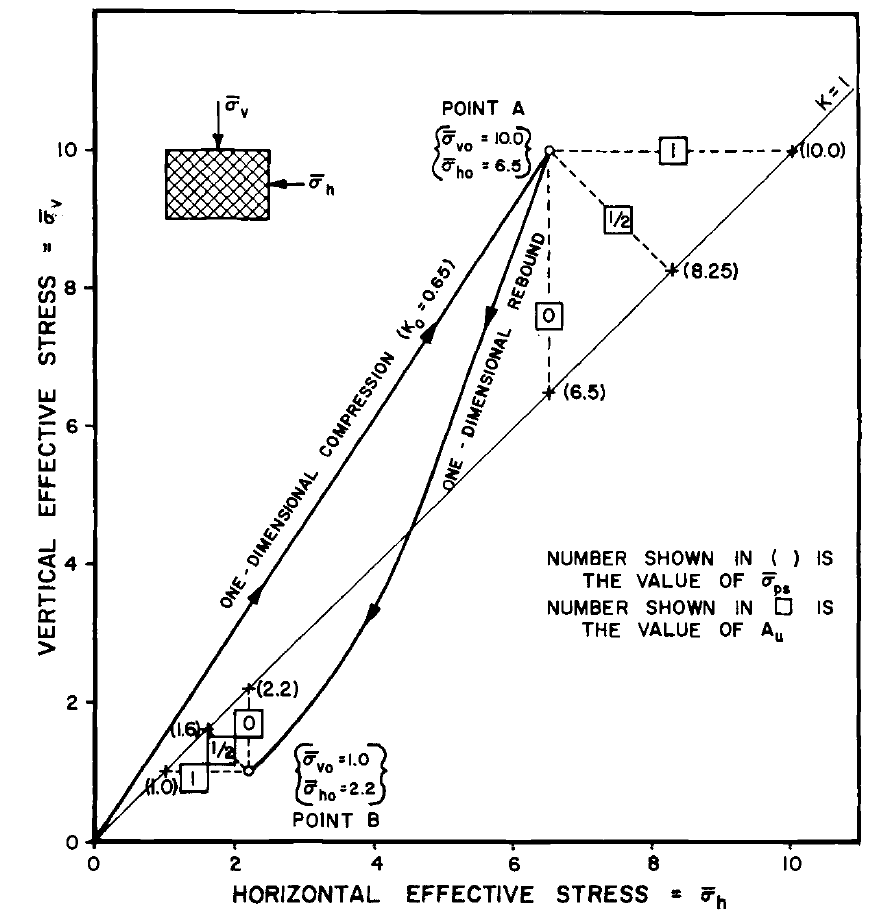
\includegraphics[width=0.5\textwidth]{figures/figure-1.png}\\
    The one-dimensional compression and rebound curves simulate $K_0$ data for the London clay \citet{Skempton1961351}. \\
    一维压缩和回弹曲线模拟了伦敦黏土citet{Skempton1961351}的$K_0$数据。
    \caption{Perfect Sampling of a Normally Consolidated Clay and an Over-consolidated Clay.}
    \addtocounter{figure}{-1}
    \vspace{-5pt}
    \renewcommand{\figurename}{图}
    \caption{正常固结土和超固结土的完美采样。}
    \renewcommand{\figurename}{Figure}
    \label{figure:1}
\end{figure}